\subsection{LASSO}
\begin{frame}{Some Fancy Results}
    The plot of $\Delta_k$: 
    \begin{figure}[h]
        \centering
        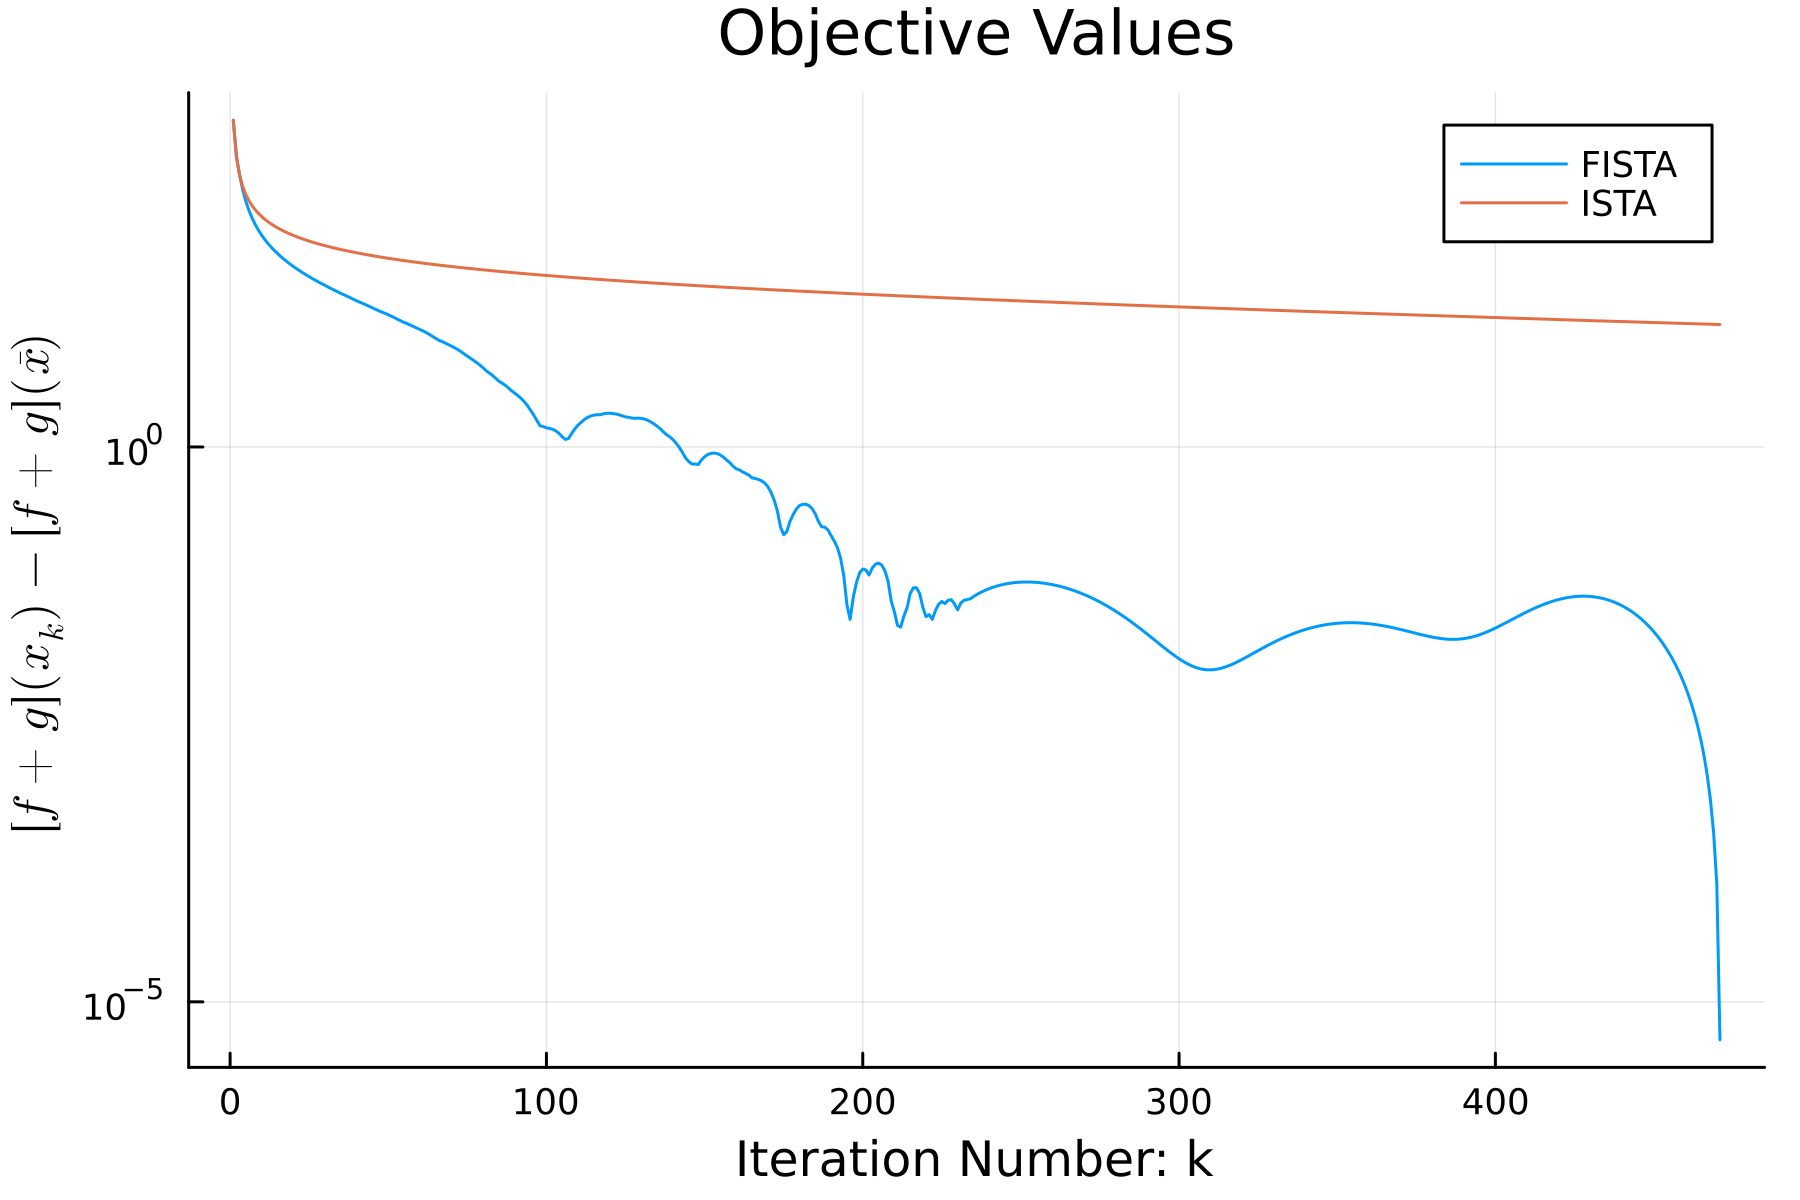
\includegraphics[width=8cm]{Assets/simple_lass_obj.png}
        \caption{The left is the objective value of the function during all iterations.}
    \end{figure}
\end{frame}

\begin{frame}{Results}
    The plot of $\Vert y^{(k)} - x^{(k + 1)}\Vert_\infty$:
    \begin{figure}[h]
        \centering
        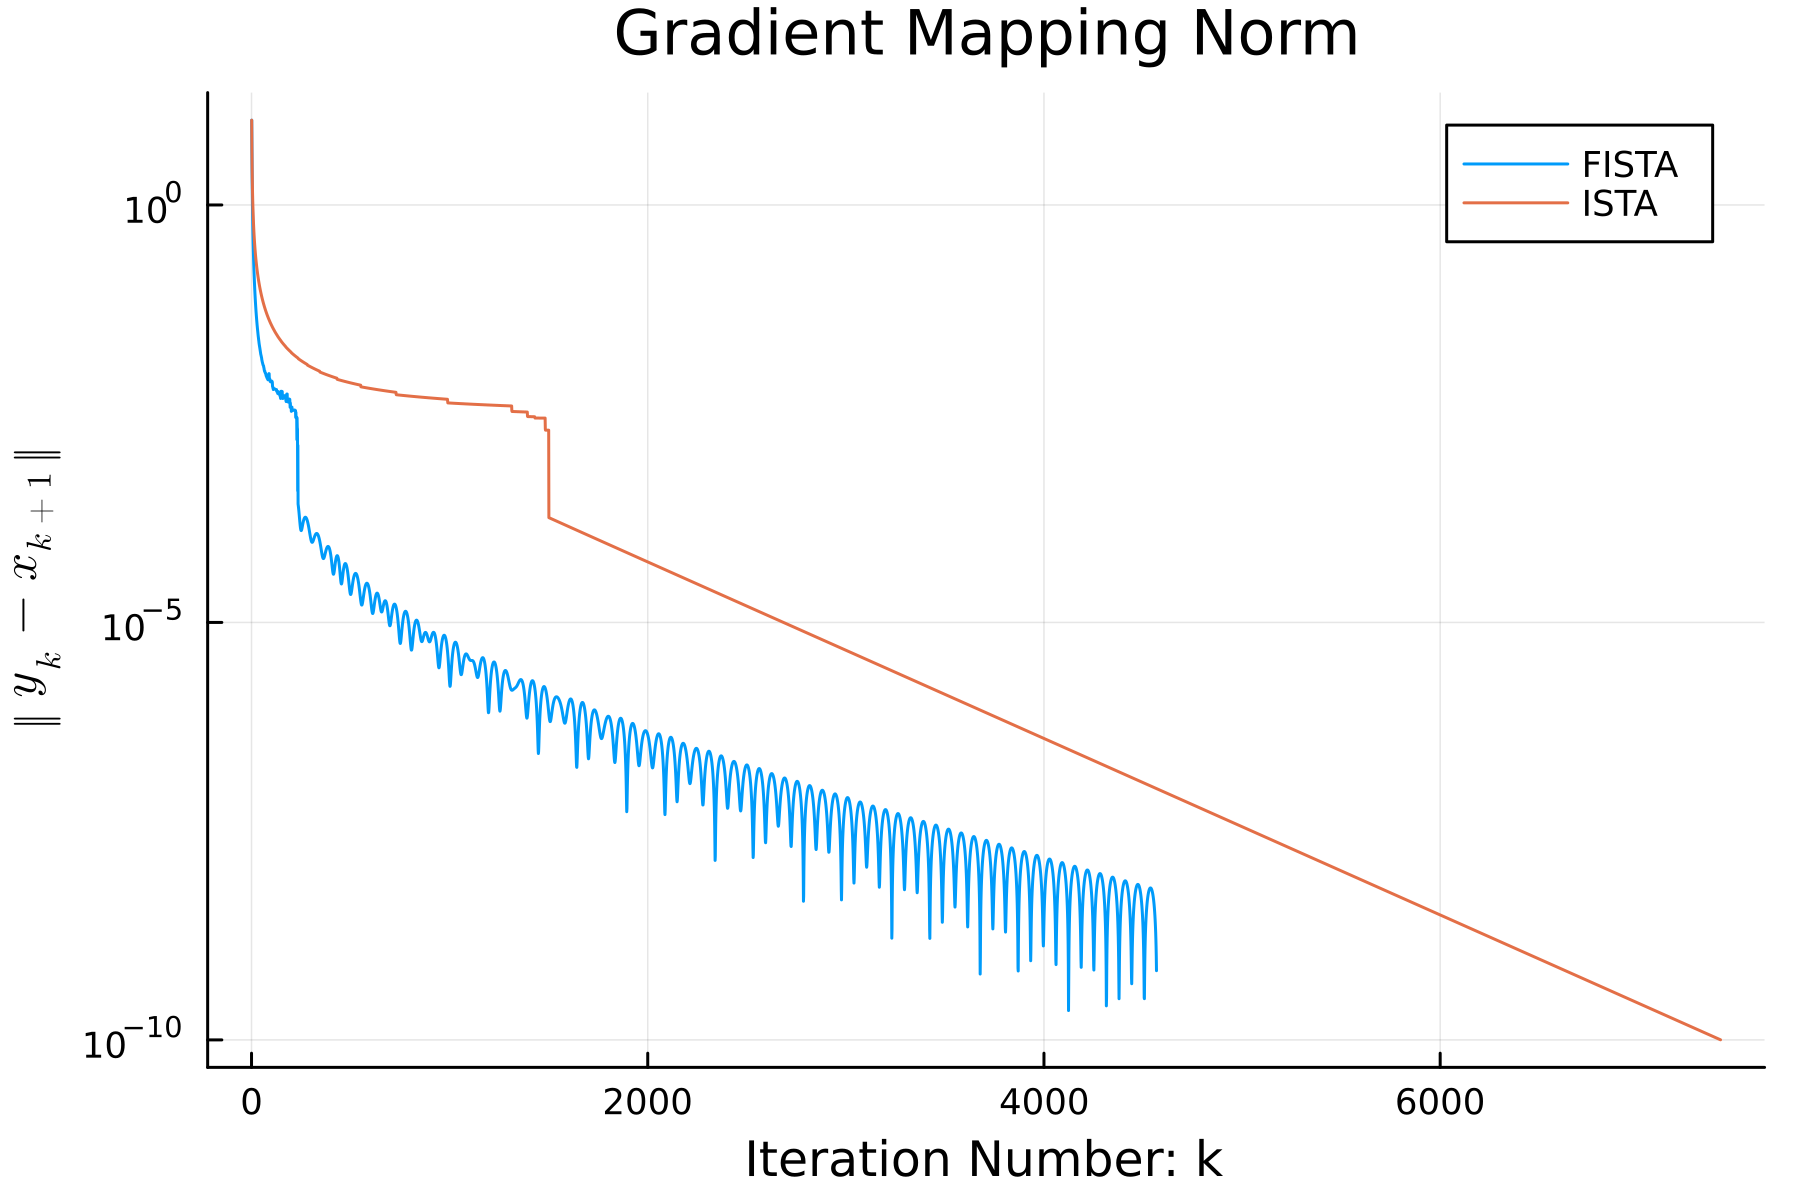
\includegraphics[width=8cm]{Assets/simple_lass_pgrad.png}
    \end{figure}
\end{frame}

\subsection{Image Deconvolution with Noise}
\begin{frame}{Experiment Setup}
    Given an image that is convoluted by a Guassian kernel with some guassian noise, we want to recover the image, given the parameters for convolutions. 
    \begin{itemize}
        \item [1.] Guassian blur with a discrete 15 by 15 kernel is a linear transform represented by a sparse matrix $A$ in the computer. 
        \item [2.] When an image is 500 by 500 with 3 color channels, $A$ is $750000 \times 750000$. 
        \item [3.] Let the noise be on all normalized colors values with $N(0, 10^{-2})$
        \item [4.] We let $\lambda = \alpha\times (3\times500^2)^{-1}$. 
        \item [5.] Implemented in Julia, and the code is too long to be shown here. 
    \end{itemize}        
\end{frame}
\begin{frame}{One Big Image for Some Fancy Results}
    We consider blurring the image of a pink unicorn that I own. 
    \begin{figure}[H]
        \centering
        
\includegraphics[width=5cm]{Assets/blurred_img.jpg}
        \caption{The image is blurred by the Gaussian Blurred matrix $A$ with a tiny amount of noise on the level of $2\times 10^{-2}$ that is barely observable. Zoom in to observe the tiny amount of Gaussian noise on top of the blur.}
        \label{fig:blurred_alto}
    \end{figure}
\end{frame}
\begin{frame}{Moer Image to Show Impressive Results}
    \begin{figure}
        \subfloat[Graph 1]{
            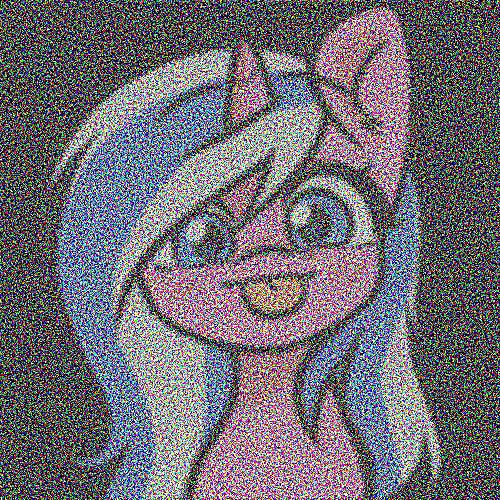
\includegraphics[width=3cm]{Assets/inverse_linear_experiment1-soln_img.jpg}
            \label{fig:1a}
        }
        \subfloat[Graph 2]
        {
            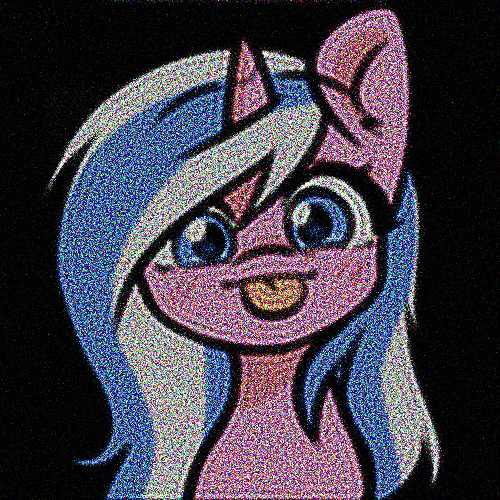
\includegraphics[width=3cm]{Assets/inverse_linear_experiment2-soln_img.jpg}
            \label{fig:1b}
        }
        \subfloat[Graph 3]
        {
            
\includegraphics[width=3cm]{Assets/inverse_linear_experiment3-soln_img.jpg}
            \label{fig:1c}
        }
        \caption{(a) $\alpha = 0$, without any one norm penalty, is not robust to the additional noise. (b) $\alpha = 0.01$, there is a tiny amount of $\lambda$. (c) $\alpha = 0.1$, it is more penalty compared to (a).}
        \label{fig:alto_deblurred}
    \end{figure}

\end{frame}